% Template:     Informe LaTeX
% Documento:    Archivo principal
% Versión:      8.2.7 (21/08/2023)
% Codificación: UTF-8
%
% Autor: Pablo Pizarro R.
%        pablo@ppizarror.com
%
% Manual template: [https://latex.ppizarror.com/informe]
% Licencia MIT:    [https://opensource.org/licenses/MIT]

% CREACIÓN DEL DOCUMENTO
\documentclass[
	spanish, % Idioma: spanish, english, etc.
	letterpaper, oneside
]{article}

\usepackage{multirow}
\usepackage{caption}



% INFORMACIÓN DEL DOCUMENTO
\def\documenttitle {Tarea 2 Data Science for Social Network Analysis}
\def\documentsubtitle {}
\def\documentsubject {}

\def\documentauthor {Bryan Cabezas}
\def\coursename {}
\def\coursecode {IN7600}

\def\universityname {Universidad de Chile}
\def\universityfaculty {Facultad de Ciencias Físicas y Matemáticas}
\def\universitydepartment {Departamento de Ingeniería Industrial}
\def\universitydepartmentimage {departamentos/dii}
\def\universitydepartmentimagecfg {height=1.57cm}
\def\universitylocation {Santiago de Chile}

% INTEGRANTES, PROFESORES Y FECHAS
\def\authortable {
	\begin{tabular}{ll}
		Integrantes:
		& \begin{tabular}[t]{l}
			Bryan Cabezas Sandoval\\
		\end{tabular} \\
		Profesor:
		& \begin{tabular}[t]{l}
            Richard Weber
		\end{tabular} \\
		Auxiliar:
		& \begin{tabular}[t]{l}
			Dimitri Loaiza \\
            Susana Rojas
		\end{tabular} \\
		Ayudantes:
		& \begin{tabular}[t]{l}
			Víctor Bunster
		\end{tabular} \\
		& \\
		\multicolumn{2}{l}{Fecha de entrega: 24 de Abril del 2026} \\
		\multicolumn{2}{l}{\universitylocation}
	\end{tabular}
}

% IMPORTACIÓN DEL TEMPLATE
\input{template}
%\usepackage[a4paper,margin=2.5cm]{geometry}
% INICIO DE PÁGINAS
\begin{document}
% PORTADA
\templatePortrait

% CONFIGURACIÓN DE PÁGINA Y ENCABEZADOS
\templatePagecfg

% --- AQUÍ AGREGAS EL ÍNDICE ---
\newpage % Opcional: para que el índice empiece en una página nueva
\tableofcontents
\newpage % Opcional: para que tu contenido empiece después del índice
% ------------------------------


% CONFIGURACIONES FINALES
\templateFinalcfg
% ======================= INICIO DEL DOCUMENTO =======================




\section{Sección 1 Métodos clasicos}
\subsection{1.1}
Se crea una visualización de la red de Polimá Westcoast mediante Pyvis, utilizada en la tarea 1.

\begin{figure}[ht!]
    \centering
    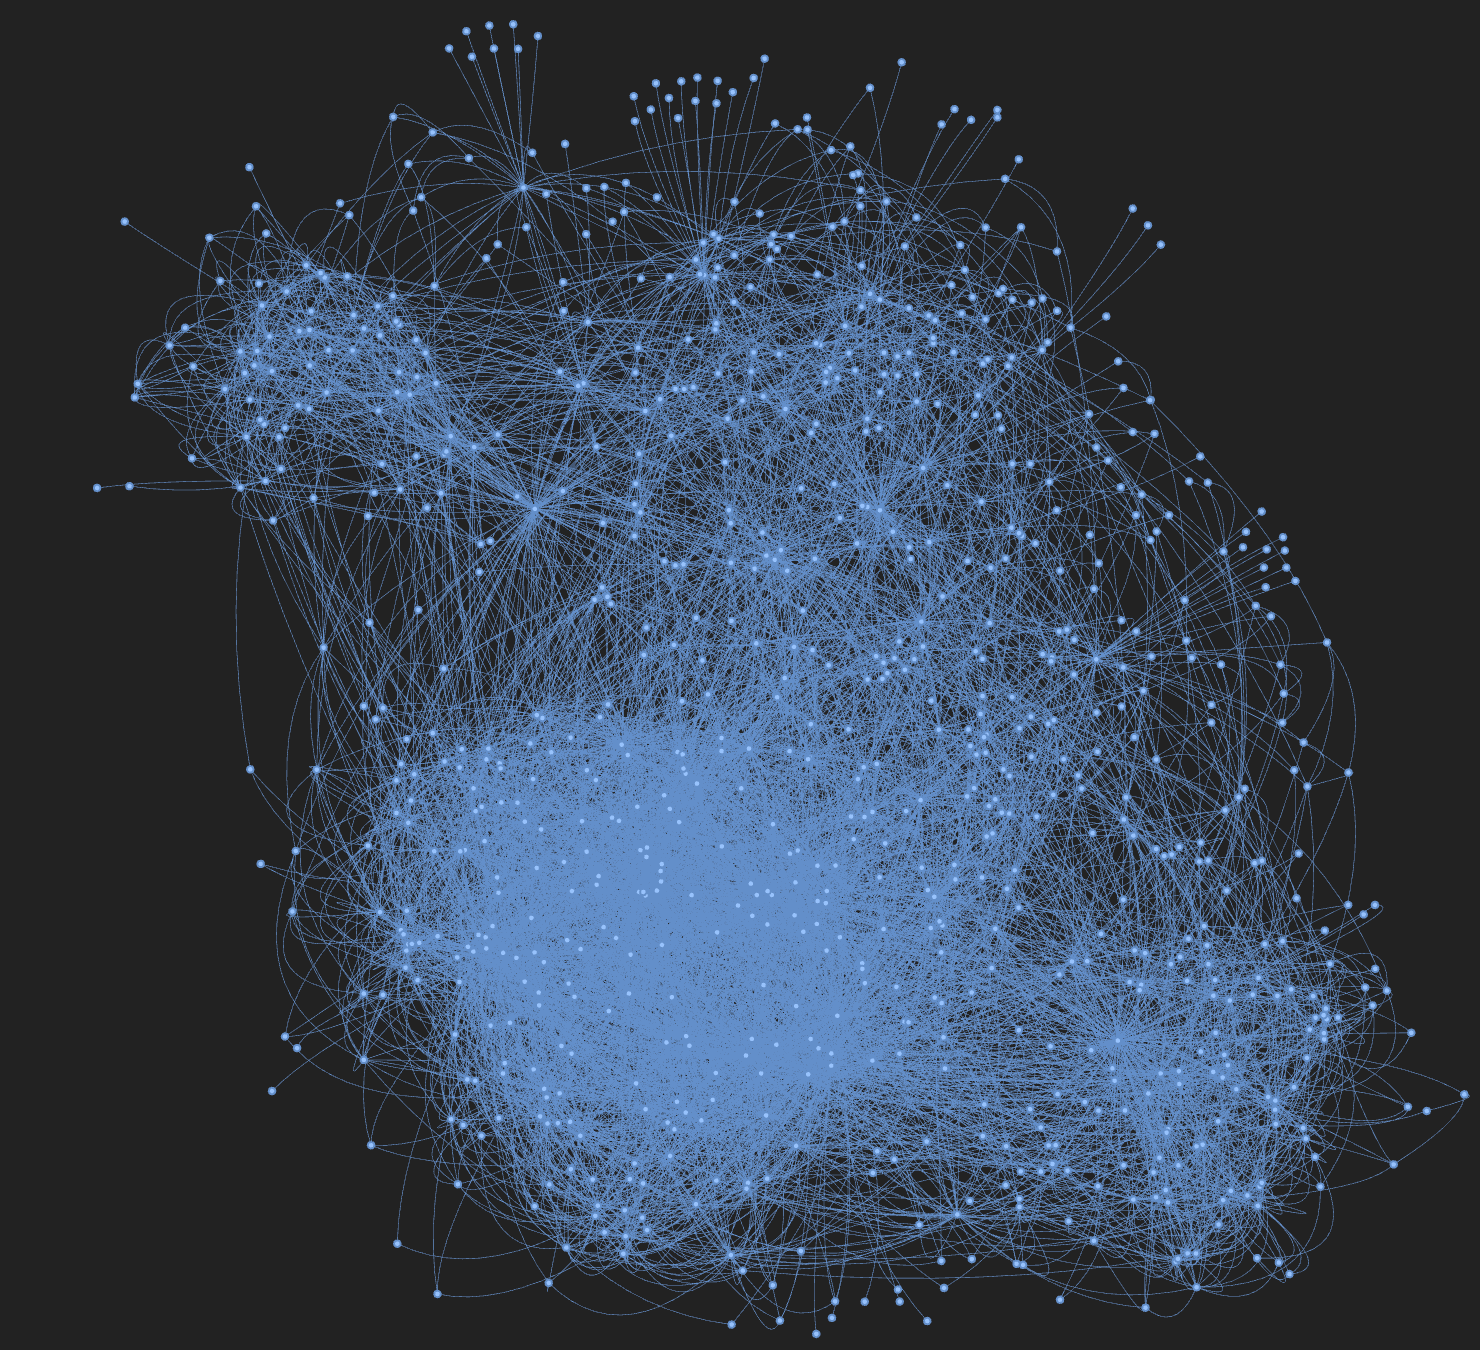
\includegraphics[width=0.7\textwidth]{img/Tarea/1.1.png}
    \caption{Social Network de Polimá Westcoast con Pyvis}
    \label{fig:PolimaWestcoast}
\end{figure}


\subsection{1.2 y 1.3}
Se presenta la visualización de la detección de comunidades mediante el algoritmo Girvan-Newman en la figura \ref{fig:PolimaGirvanNewman}, el cual detecto únicamente 2 comunidades. Por otro lado, el algoritmo de Louvain detectó 6 comunidades, lo que sugiere una estructura más compleja y diversa dentro de la red. Esto se puede observar en la figura \ref{fig:PolimaLouvain}. Asimismo, Louvain presenta una división más clara entre las comunidades, mientras que Girvan-Newman muestra una división más difusa, lo que sugiere que el algoritmo de Louvain es más efectivo para detectar comunidades en esta red específica. Además, el algoritmo de Louvain es más eficiente en términos de tiempo de ejecución, demorando segundos, mientras que el algoritmo de Girvan-Newman se demoro 42 minutos en ejecutarse.  

\begin{figure}[ht!]
    \centering
    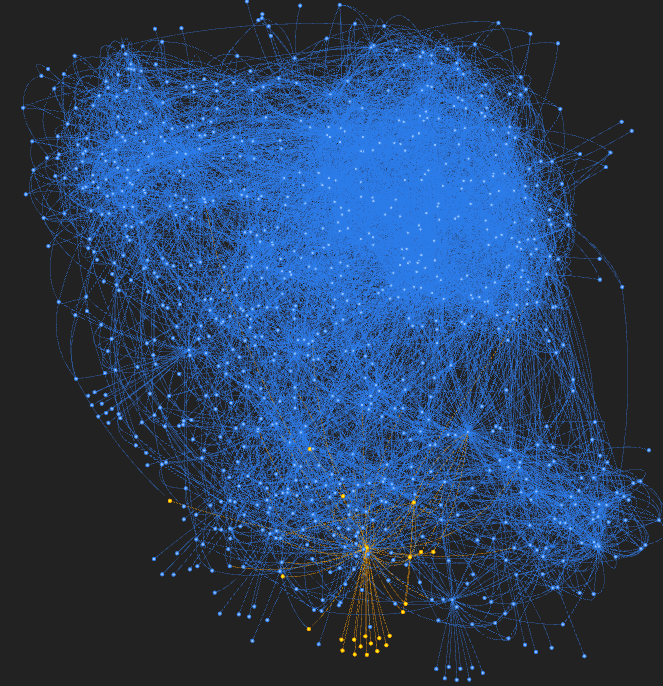
\includegraphics[width=0.7\textwidth]{img/Tarea/PolimaGirvanNewman.png}
    \caption{Social Network de Polimá Westcoast con comunidades detectadas por Girvan-Newman en Pyvis}
    \label{fig:PolimaGirvanNewman}
\end{figure}

\begin{figure}[ht!]
    \centering
    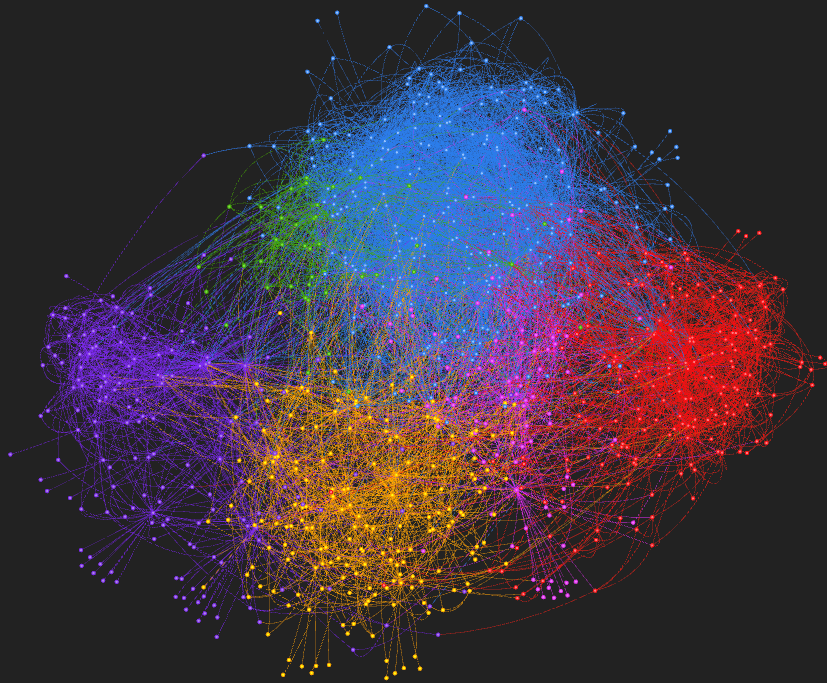
\includegraphics[width=0.7\textwidth]{img/Tarea/PolimaLouvain.png}
    \caption{Social Network de Polimá Westcoast con comunidades detectadas por Louvain en Pyvis}
    \label{fig:PolimaLouvain}
\end{figure}

\newpage

\subsection{1.4}
Se presenta la comunidad 0 en la figura \ref{fig:Comunidad0Louvain}, la comunidad 1 en la figura \ref{fig:Comunidad1Louvain} y la comunidad 2 en la figura \ref{fig:Comunidad2Louvain}. 

Se observa que la comunidad 0, la cual presenta mayor cantidad de artistas (239), se caracteriza por una fuerte presencia de artistas de trap latino, reggaeton y latin hip hop, lo que sugiere una comunidad centrada en el género urbano latinoamericano. La cantidad elevada en esta comunidad se explica debido que nacio de la red de pólima westcoast, quien es un artista chileno de trap latino, evidenciando una fuerte cohesión en torno al género urbano.

La comunidad 1, con 177 artistas, presenta un patron similar de géneros urbanos, pero siendo el genero con mayor cantidad de integrantes el de trap argentino, lo que sugiere una comunidad más enfocada en la escena musical argentina. Esto se repite en la cuarta posición de la comunidad, que destaca el hip hop argentino, lo que refuerza el patron. Aún asi, esta comunidad también presenta vínculos con la presencia de artistas latinos, incluido algunos de trap venezolano y hip hop mexicano, indicando intercambio cultural.

Finalmente, la comunidad 2, compuesta por 176 artistas, se aleja del nicho urbano, presentando un patrón más hacia un enfoque de géneros internacionales y comerciales, como es el pop, dance pop, pop rap, y subgéneros elctrónicos como electro house y tropical house, lo que sugiere una comunidad más orientada hacia el mercado global y anglosajón. Esta comunidad se creo posiblemente a colaboraciones de artistas latinos con artistas de pop global y eléctronica.



\begin{figure}[ht!]
    \centering
    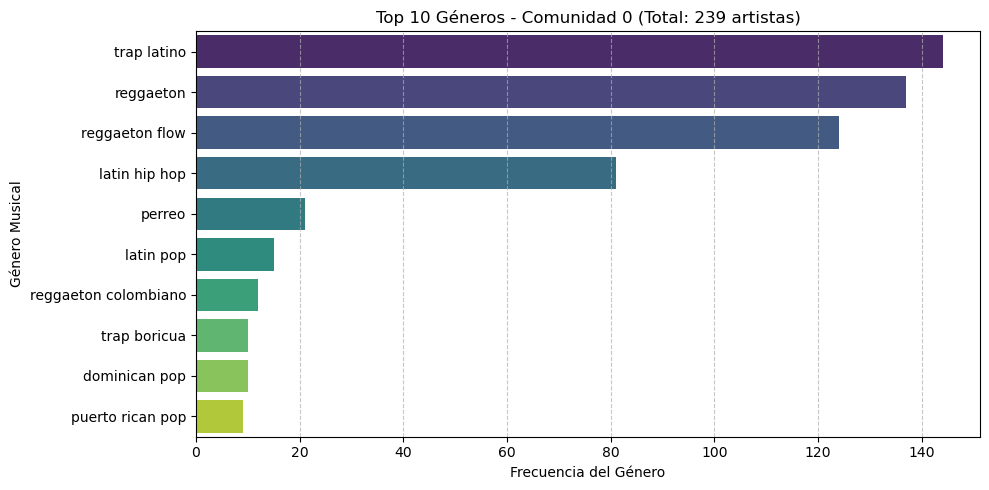
\includegraphics[width=0.7\textwidth]{img/Tarea/1.4 Comunidad 0.png}
    \caption{Top 10 géneros más repetidos en la comunidad 0 detectada por Louvain}
    \label{fig:Comunidad0Louvain}
\end{figure}

\begin{figure}[ht!]
    \centering
    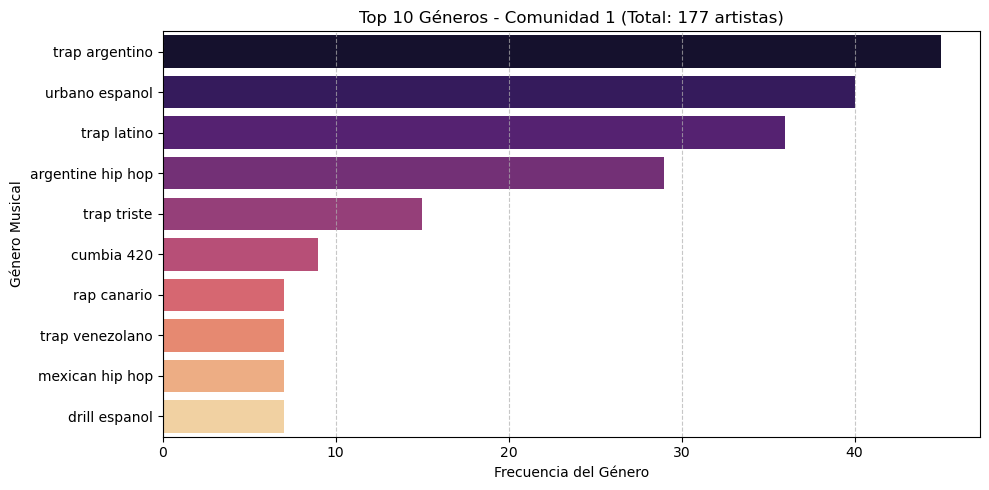
\includegraphics[width=0.7\textwidth]{img/Tarea/1.4 Comunidad 1.png}
    \caption{Top 10 géneros más repetidos en la comunidad 1 detectada por Louvain}
    \label{fig:Comunidad1Louvain}
\end{figure}

\begin{figure}[ht!]
    \centering
    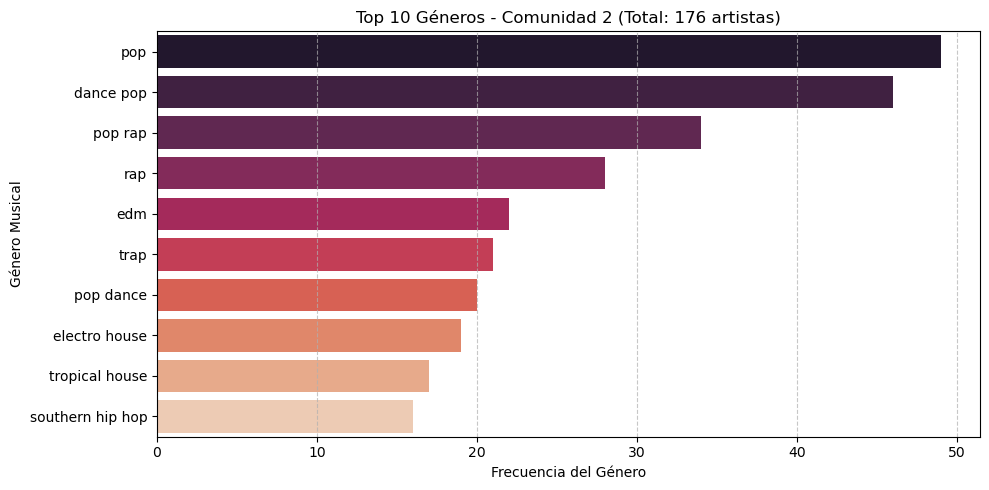
\includegraphics[width=0.7\textwidth]{img/Tarea/1.4 Comunidad 2.png}
    \caption{Top 10 géneros más repetidos en la comunidad 2 detectada por Louvain}
    \label{fig:Comunidad2Louvain}
\end{figure}


\section{Sección 2 Embeddings}

\subsection{2.1}
El método de embeddings basado en caminata aleatoria (random walks), como DeepWalk, funciona generando secuencias de nodos a través de caminatas aleatorias en el grafo. Es decir, por cada nodo en el grafo, se realizan múltiples caminatas aleatorias de longitud fija, lo que produce una serie de "sentencias" de nodos. Luego, estas secuencias se tratan como si fueran frases en un corpus de texto (utilizando técnicas de procesamiento de lenguaje natural), de forma que se aplica skip-gram para aprender representaciones vectoriales de los nodos, de manera que nodos que aparecen en contextos similares (que co-ocurren en las caminatas varias veces) tendrán representaciones vectoriales similares, lo que permite capturar la estructura del grafo. Esta representación vectorial saliente son los embeddings.

\subsection{2.2}
Aplique este método a su red y muestre sus resultados en dos dimensiones usando una
técnica de reducción de dimensionalidad. ¿Qué significa que dos nodos estén cerca?


Se presenta la visualización de los embeddings de DeepWalk utilizando t-SNE en la figura \ref{fig:EmbeddingsT-SNE}.  En esta visualización, cada punto representa un nodo (artista) en el espacio de embeddings reducido a dos dimensiones. La cercanía entre dos nodos en esta visualización indica que sus representaciones vectoriales son similares a nivel local, lo que sugiere que estos nodos tienen patrones de conexión similares en el grafo original. En otras palabras, si dos nodos están cerca en el espacio de embeddings, es probable que compartan vecinos comunes o tengan roles similares dentro de la red, lo que puede reflejar similitudes en términos de colaboraciones y comunidades, donde artistas que pertencen a un mismo género o circulo aparecen representados en proximidad. Sin embargo, es importancia destacar que t-SNE es eficaz para preservar las relaciones de vecindad cercana, pero las distancias a gran escala entre clusters no reflejan una métrica de distancia global exacta. Asimismo, se generó una visualización proyectada con t-SNE, pero asignando colores a los nodos según las comunidades detectadas por Louvain en la figura \ref{fig:EmbeddingsT-SNE-Louvain}, evidenciando que los nodos dentro de una misma comunidad tienden a agruparse juntos en el espacio de embeddings, lo que sugiere que el método de embeddings captura efectivamente la estructura comunitaria de la red.



\begin{figure}[ht!]
    \centering
    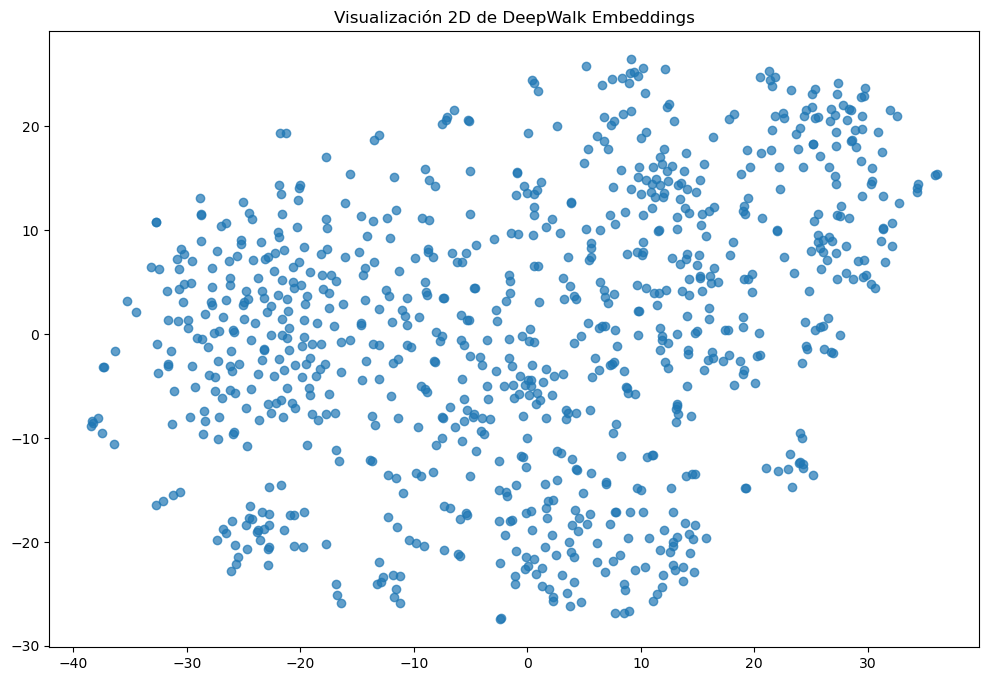
\includegraphics[width=0.7\textwidth]{img/Tarea/EmbeddingsT-SNE.png}
    \caption{Visualización 2D de DeepWalk Embeddings utilizando t-SNE}
    \label{fig:EmbeddingsT-SNE}
\end{figure}

\begin{figure}[ht!]
    \centering
    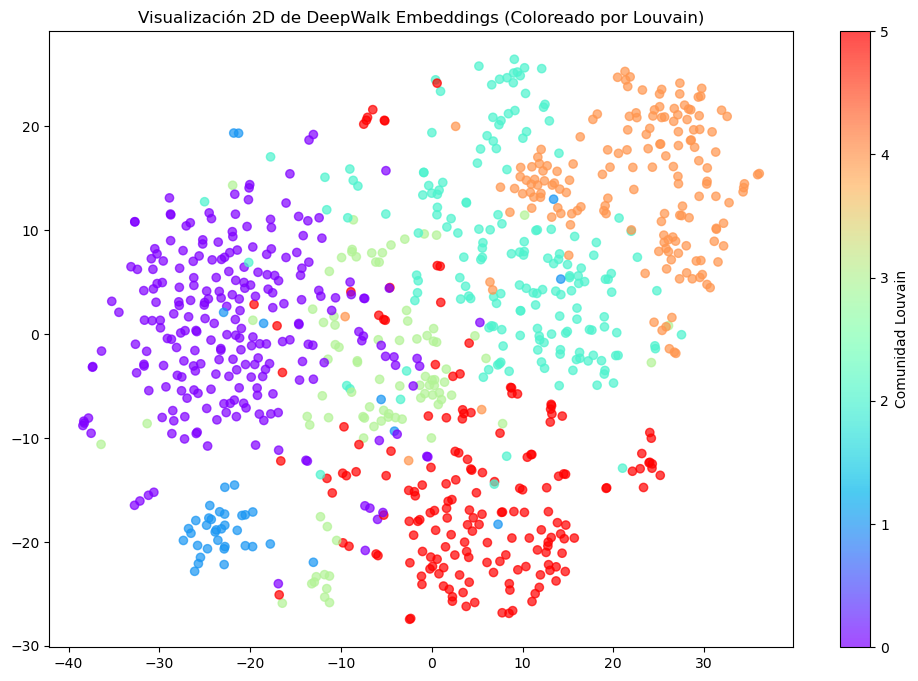
\includegraphics[width=0.7\textwidth]{img/Tarea/EmbeddingsT-SNELouvain.png}
    \caption{Visualización 2D de DeepWalk Embeddings utilizando t-SNE con colores según comunidades de Louvain}
    \label{fig:EmbeddingsT-SNE-Louvain}
\end{figure}

\subsection{2.3}
Se decidio aplicar el método de clustering K-means sobre los embeddings de DeepWalk para generar comunidades. El algoritmo K-means se basa en la idea de particionar los datos en K clusters, en este caso, se decidio crear 6 clusters para mantener la misma cantidad de comunidades detectadas por el algoritmo de Louvain. El algoritmo asigna cada nodo a uno de los clusters basandose en la distancia euclidiana entre el nodo y el centroide del cluster, de manera que nodos con embeddings similares (que están cerca en el espacio de embeddings) serán agrupados juntos. Este método permite identificar grupos de nodos que comparten patrones similares, pero asume que los clusters son esféricos y de tamaño similar. El resultado de aplicar K-means sobre los embeddings se presenta en la figura \ref{fig:EmbeddingsKMeans}, donde cada color representa un cluster diferente. 

\begin{figure}[ht!]
    \centering
    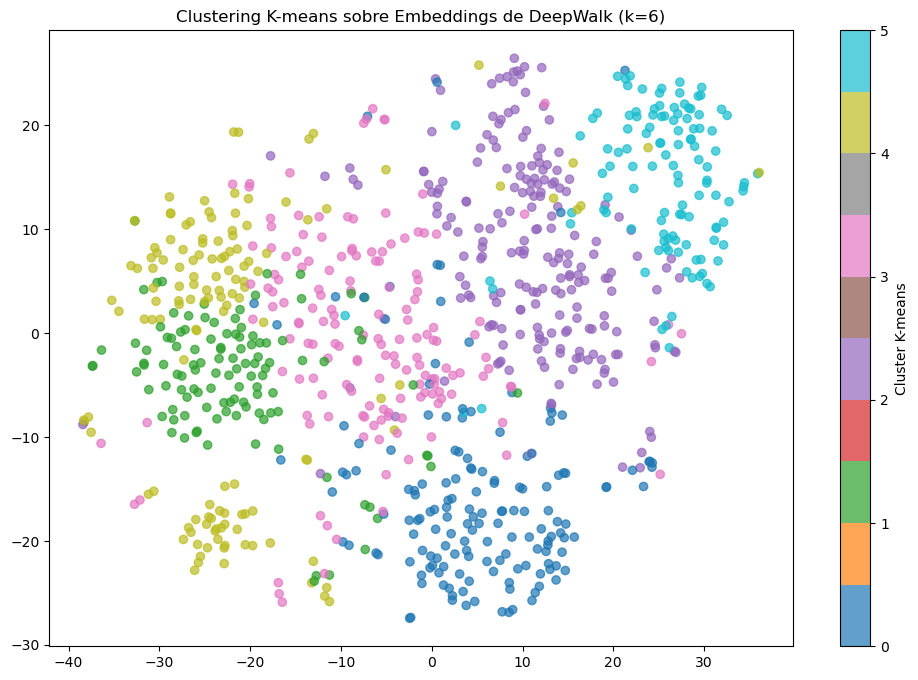
\includegraphics[width=0.7\textwidth]{img/Tarea/ClusteringKmeansDeepWalk.png}
    \caption{Visualización 2D de DeepWalk Embeddings con clusters generados por K-means}
    \label{fig:EmbeddingsKMeans}
\end{figure}


\subsection{2.4}
Se presentan las 3 comunidades con más artistas ordenadas de mayor a menor, siendo el cluster 2 el que presenta mayor cantidad de aristas (203), seguido por el cluster 3 (159) y el cluster 0 (156). Se presentan los histogramas de los 10 géneros más repetidos en cada comunidad en las figuras \ref{fig:KMeansCluster2}, \ref{fig:KMeansCluster3} y \ref{fig:KMeansCluster0} respectivamente. 

Se observa que el cluster 2 presenta un pátron similar a la comunidad 1 detectada por Louvain, con una fuerte presencia de géneros urbanos argentinos, pero con un aumento sustancial en artistas detectados del género urbano español, incluyendo artistas uruguayos. Esto demuestra que los aristas asignados para cada cluster son distintos a los artistas asignados por Louvain, capturando estructura diferente en la red. 

En el cluster 3, el segundo cluster con mayor cantidad de artistas, muestra un patrón similar a la comunidad 0 de Louvain, con una fuerte presencia de géneros urbanos latinos, pero con un aumento en artistas del género reggaeton y latin pop, superando al trap latino, sugiriendo una comunidad más orientada hacia ambos géneros. Además, se observa géneros nuevos en este cluster, como el colombian pop, mexican pop y el spanish pop, mostrando una generalización entre artistas de reggaeton y pop latino. 

Finalmente, el cluster 0, con la menor cantidad de artistas entre los tres, muestra un patron igual a la comunidad 2 de Louvain, con una fuerte presencia de géneros internacionales y comerciales, como el pop, dance pop, pop rap y subgéneros electrónicos. Asimismo, en este cluster se observa un diferencia muy menor entre artistas del género pop y dance pop, lo que puede indicar que existen artistas que se encuentran en la frontera entre ambos géneros.

Cabe mencionar que la comunidad más grande detectada por K-means sean de artistas del género urbano también se explica por la presencia de Polimá Westcoast, quien es un artista chileno de trap latino, lo que sugiere que el método de embeddings y clustering K-means capturó efectivamente la estructura de la red en torno a este artista y su género musical.

\begin{figure}[ht!]
    \centering
    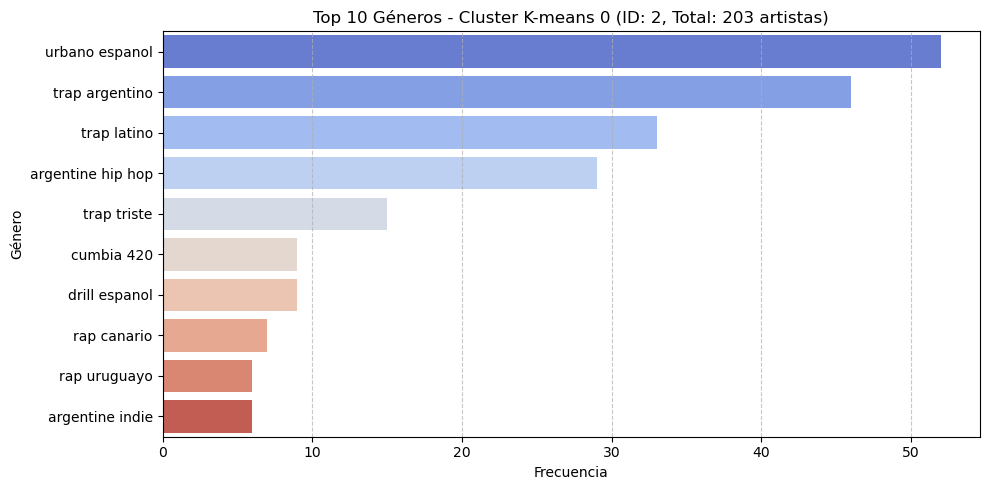
\includegraphics[width=0.7\textwidth]{img/Tarea/1.OrdenadoK-means.png}
    \caption{Top 10 géneros más repetidos en el cluster 2 generado por K-means}
    \label{fig:KMeansCluster2}
\end{figure}

\begin{figure}[ht!]
    \centering
    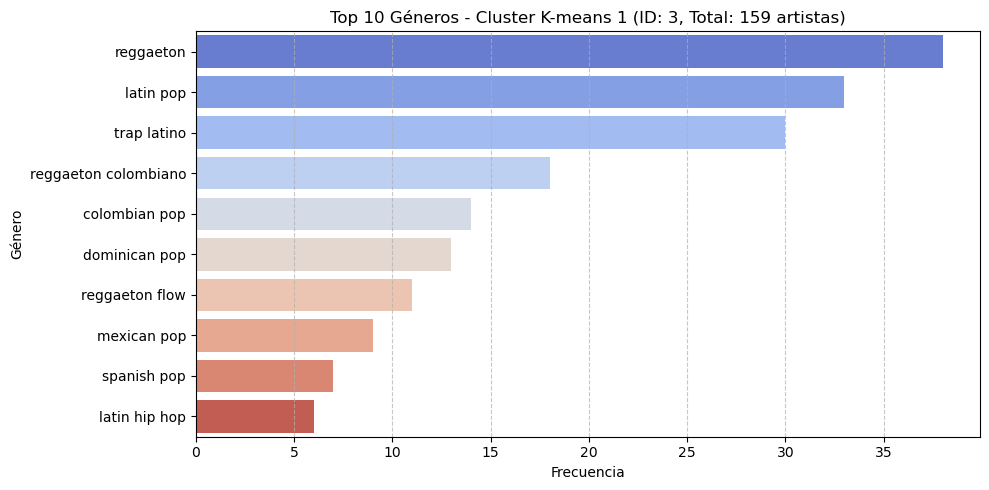
\includegraphics[width=0.7\textwidth]{img/Tarea/2.OrdenadoK-means.png}
    \caption{Top 10 géneros más repetidos en el cluster 3 generado por K-means}
    \label{fig:KMeansCluster3}
\end{figure}

\begin{figure}[ht!]
    \centering
    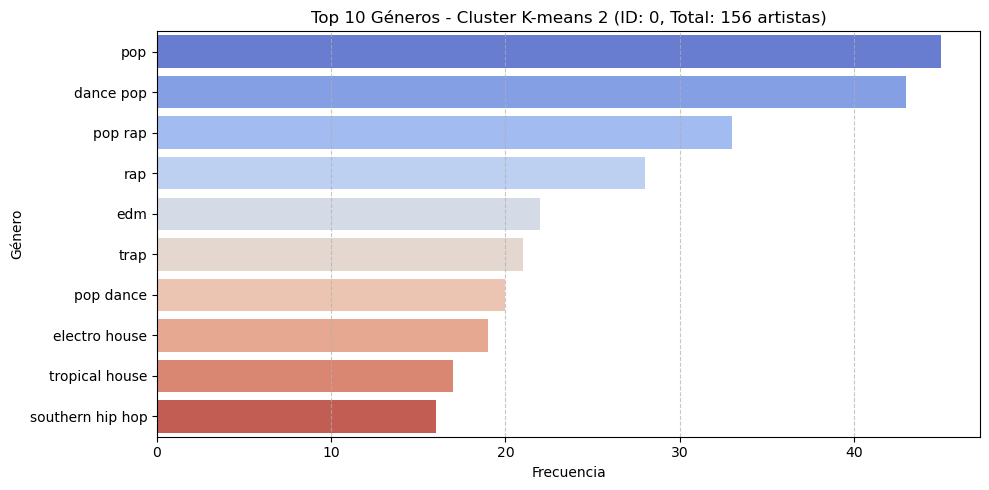
\includegraphics[width=0.7\textwidth]{img/Tarea/3.OrdenadoK-means.png}
    \caption{Top 10 géneros más repetidos en el cluster 0 generado por K-means}
    \label{fig:KMeansCluster0}
\end{figure}


\subsection{2.5}
2.5 Compare los resultados obtenidos en esta sección con los resultados obtenidos en la
sección anterior y comente

Los resultados obtenidos en la sección de detección de comunidades utilizando el método Louvain y el método de embeddings con clustering K-means muestran similitudes y diferencias en la estructura comunitaria de la red. Por un lado, al observar las visualizaciones de los embeddings con t-SNE, se puede visualizar que las comunidades detectadas cambian según el metodo utilizado, lo que sugiere que cada método captura diferentes aspectos de la estructura de la red. Se visualiza que K-means tiende a generar clusters más pequeños y con menos puntos en comparación con Louvain, lo que sugiere que K-means puede estar capturando subcomunidades dentro de las comunidades más grandes detectadas por Louvain. Esto no se repite en todos los clusters, pero si en la comunidad de color morado, donde Louvain detecta una comunidad grande, mientras que K-means la divide en dos clusters más pequeños, de color verde y amarillo. Además, al analizar los géneros más repetidos en cada comunidad, se observa que ambos métodos identifican comunidades con patrones similares de géneros musicales, pero con diferencias en la composición de los artistas dentro de cada comunidad. Por ejemplo, el cluster 2 de K-means muestra una mayor presencia de artistas del género urbano español, junto con la incorporación de artistas uruguayos, lo que no se observa en la comunidad 1 de Louvain, aún asi enfatiza la presencia de artistas del género urbano argentino, incorporando artistas de argetine indie. Por otro lado, el cluster 3 de K-means muestra una mayor presencia de artistas del género reggaeton y pop latino, lo que sugiere una comunidad más orientada hacia ambos géneros, mientras que la comunidad 0 de Louvain, que es la más similar, se enfoca en el trap latino. Asimismo, los tamaños de las comunidades detectados por K-means son menores en comparación con Louvain, lo que respalda la idea de que K-meas puede estar capturando subcomunidades. Además, se observa el cluster 0 de K-means, muestra un patron similar a la comunidad 2 de Louvain, con una fuerte presencia de géneros internacionales y comerciales, pero con una diferencia muy menor entre la cantidad de artistas del género pop y dance pop, teniendo una menor diferencia entre ambos géneros en la detección de K-means. 

En general, ambos métodos identifican comunidades con patrones similares de géneros musicales, pero cada uno lo hace con técnicas de detección de comunidades diferentes, capturando diferentes aspectos de la estructura de la red, resaltando la importancia de utilizar múltiples enfoques para comprender la complejidad de las redes sociales y las comunidades dentro de ellas.



 


\end{document}
